\documentclass[11pt]{article}
\usepackage[margin=1in]{geometry}
\usepackage{amsmath,amssymb}
\usepackage{booktabs}
\usepackage{multirow}
\usepackage{graphicx}
\usepackage[hidelinks]{hyperref}
\usepackage{xcolor}
\usepackage{microtype}
\usepackage{tikz}
\usetikzlibrary{arrows.meta,positioning,fit,calc,decorations.pathreplacing}
\definecolor{gcol}{HTML}{E8742C}
\definecolor{pcol}{HTML}{2F9C86}
\definecolor{ink}{HTML}{2B2F2E}
\setlength{\emergencystretch}{2em}

\title{PartLock: Strictly Local Hierarchical Motion Tokens\\for Endless, Switchable Text-to-Motion Streaming}
\author{Kaiji Hiruma\\ \small Independent Researcher}
\date{}

\newcommand{\gtok}{g}
\newcommand{\ptok}{p}

\begin{document}
\maketitle

\begin{abstract}
I present \emph{PartLock}, a streaming text-to-motion system that generates 3D human motion
without end, switches between actions without returning to a rest pose, and makes per-body-part
control \emph{structurally} local.
Its core is a hierarchical, strictly causal motion tokenizer: every four frames are encoded into one
whole-body (global) token and six body-part tokens, and each body part is decoded \emph{only} from the
global token and its own part token.
This factorization gives a structural guarantee:
replacing the tokens of one part changes that part and nothing else (measured change in all other
parts: exactly $0$), while the shared global token carries whole-body coordination.
All convolutions are causal, so streaming decoding equals whole-sequence decoding
(max.\ difference $2.1\times10^{-15}$ in float64).
On top of the tokenizer, a 30.5M-parameter decoder-only Transformer generates the seven tokens of each
step from CLIP text features, added at every token position, and runs for 60\,s with no degradation.
Finally, a simple switching rule---on a text change, keep only the last step of the context---lets the
motion change action on command and stop when told, with no extra computation.
\end{abstract}

%=====================================================================
\section{Introduction}

Text-to-motion models now produce convincing clips of a few seconds.
Interactive applications---avatars, games, agents that act while they talk---need something different:
motion that \emph{never ends}, that \emph{changes action on command} without snapping back to a
standing pose, and that can be steered \emph{per body part} (``keep walking, but wave with the right
hand'').

Recent streaming generators address the first two needs~\cite{motionstreamer,dart,timelinecontrol}.
Part-level control, however, is usually obtained by letting part representations exchange information
(e.g., message passing over the skeleton graph~\cite{timelinecontrol}).
This helps coordination, but it also means that an instruction given to one part can leak into all
others, and nothing in the architecture prevents it.

I take the opposite route and make locality a property of the representation itself.
My tokenizer splits each 4-frame step into a \emph{global} token, shared by the whole body, and six
\emph{part} tokens (torso, head, right/left arm, right/left leg).
Each part is decoded from \emph{[global token, own part token]} only.
Coordination between parts is carried by the global token; locality is guaranteed because a part
decoder never sees another part's token (Fig.~\ref{fig:overview}).

\paragraph{Contributions.}
\begin{itemize}
\item \textbf{Strictly local hierarchical motion tokens.}
A global + part factorization in which per-part edits are local \emph{by construction}
(other parts change by exactly $0$), while the shared global token carries whole-body coordination
(Sec.~\ref{sec:tok}, Table~\ref{tab:checks}).
\item \textbf{A strictly causal tokenizer for streaming.}
Left-padded causal convolutions give zero look-ahead, so a motion can be decoded as it is generated,
with output identical to offline decoding (Table~\ref{tab:checks}).
\item \textbf{Endless generation with a token-level Transformer}, conditioned on text at
\emph{every token position}, so that each part's tokens can later be given their own text.
\item \textbf{A free switching rule.}
Forgetting all but the last step at a text change makes the model follow the new instruction and stop
when told, at no computational cost (Sec.~\ref{sec:switch}).
\end{itemize}

%=====================================================================
\section{Related Work}

\paragraph{Text-to-motion.}
Discrete-token models (T2M-GPT~\cite{t2mgpt}, MoMask~\cite{momask}) and diffusion models
(MDM~\cite{mdm}) generate fixed-length clips from text, typically with a non-causal tokenizer or
denoiser that needs the whole clip.

\paragraph{Streaming and long-horizon generation.}
MotionStreamer~\cite{motionstreamer} generates causal continuous latents autoregressively and introduced
the 272-dimensional HumanML3D representation I use.
DART~\cite{dart} composes short motion primitives in real time.
FlowMDM~\cite{flowmdm} produces long sequences with smooth transitions offline.

\paragraph{Part-level control.}
TimelineControl~\cite{timelinecontrol} streams motion from overlapping, part-specific instructions with a
causal part autoencoder whose part latents communicate through skeleton message passing.
ParTY~\cite{party} quantizes full-body and part motion with separate tokenizers and fuses them in the
generator.
In my design, part tokens never communicate and each part decoder receives only the global token and
its own part token, so locality is guaranteed by the architecture rather than learned, and the tokenizer
is strictly causal for streaming.

%=====================================================================
\begin{figure}[t]
\centering
\resizebox{\linewidth}{!}{%
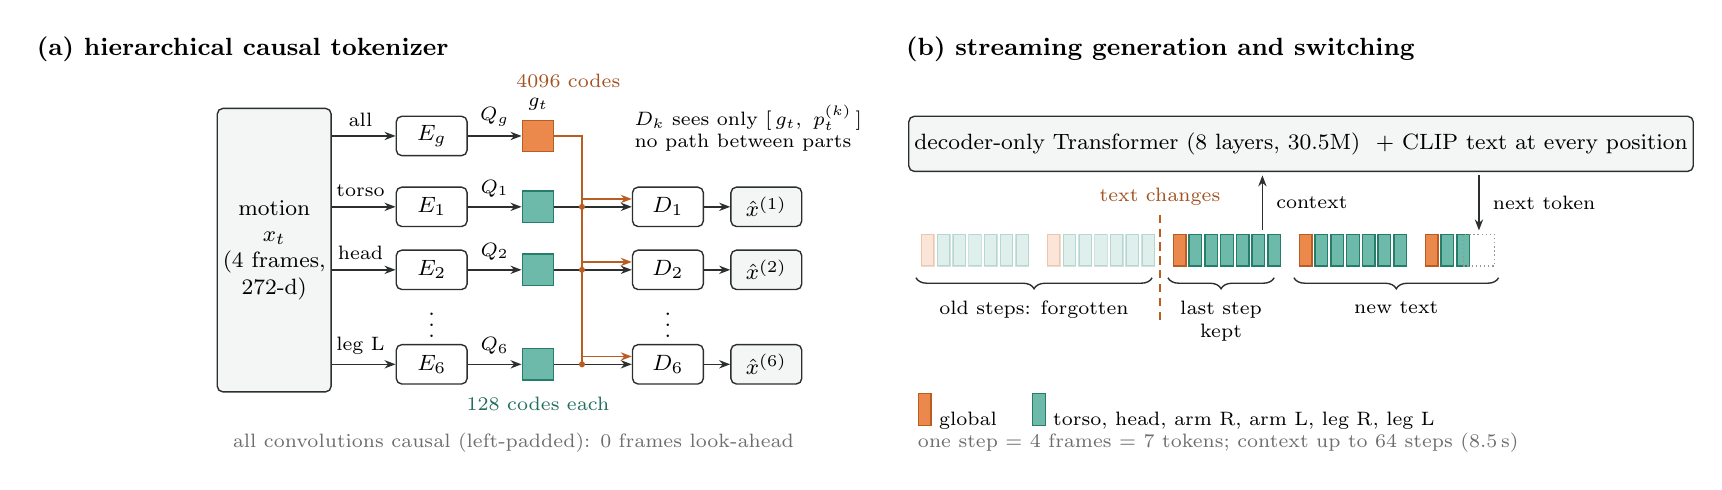
\begin{tikzpicture}[
  font=\footnotesize, >={Stealth[length=4pt]}, line width=0.5pt, draw=ink,
  box/.style={draw=ink, rounded corners=2pt, minimum height=5mm, inner sep=2pt, align=center},
  enc/.style={box, minimum width=9mm, fill=white},
  gtk/.style={draw=gcol!80!black, fill=gcol!85, minimum width=4mm, minimum height=4mm, inner sep=0pt},
  ptk/.style={draw=pcol!80!black, fill=pcol!70, minimum width=4mm, minimum height=4mm, inner sep=0pt}]

% ---------------- (a) tokenizer ----------------
\node[font=\bfseries\small] at (-0.4, 2.55) {(a) hierarchical causal tokenizer};
\node[box, minimum height=36mm, minimum width=13mm, fill=ink!5] (x) at (0,0) {motion\\$x_{t}$\\(4 frames,\\272-d)};
\node[enc] (eg) at (2.0, 1.45) {$E_g$};
\node[enc] (e1) at (2.0, 0.55) {$E_1$};
\node[enc] (e2) at (2.0,-0.25) {$E_2$};
\node      at (2.0,-0.85) {$\vdots$};
\node[enc] (e6) at (2.0,-1.45) {$E_6$};
\draw[->] (x.east |- eg) -- node[above, pos=0.45]{\scriptsize all} (eg);
\draw[->] (x.east |- e1) -- node[above, pos=0.45]{\scriptsize torso} (e1);
\draw[->] (x.east |- e2) -- node[above, pos=0.45]{\scriptsize head} (e2);
\draw[->] (x.east |- e6) -- node[above, pos=0.45]{\scriptsize leg L} (e6);

\node[gtk] (g) at (3.35, 1.45) {};
\node[font=\scriptsize] at (3.35, 1.85) {$g_t$};
\node[ptk] (p1) at (3.35, 0.55) {};
\node[ptk] (p2) at (3.35,-0.25) {};
\node[ptk] (p6) at (3.35,-1.45) {};
\draw[->] (eg) -- node[above]{\scriptsize $Q_g$} (g);
\draw[->] (e1) -- node[above]{\scriptsize $Q_1$} (p1);
\draw[->] (e2) -- node[above]{\scriptsize $Q_2$} (p2);
\draw[->] (e6) -- node[above]{\scriptsize $Q_6$} (p6);
\node[font=\scriptsize, gcol!70!black, anchor=west] at (2.95, 2.15) {4096 codes};
\node[font=\scriptsize, pcol!70!black] at (3.35,-1.95) {128 codes each};

\draw[gcol!80!black, line width=0.9pt] (g.east) -- ++(0.35,0) coordinate (bus) -- (bus |- p6);
\node[enc] (d1) at (5.0, 0.55) {$D_1$};
\node[enc] (d2) at (5.0,-0.25) {$D_2$};
\node      at (5.0,-0.85) {$\vdots$};
\node[enc] (d6) at (5.0,-1.45) {$D_6$};
\foreach \k in {1,2,6} {
  \draw[->] (p\k) -- (d\k);
  \fill[gcol!80!black] (bus |- p\k) circle (1.1pt);
  \draw[->, gcol!80!black] (bus |- p\k) ++(0,0.1) -- ($(d\k.west)+(0,0.1)$);
}
\node[box, fill=ink!5, minimum width=9mm] (y1) at (6.25, 0.55) {$\hat x^{(1)}$};
\node[box, fill=ink!5, minimum width=9mm] (y2) at (6.25,-0.25) {$\hat x^{(2)}$};
\node[box, fill=ink!5, minimum width=9mm] (y6) at (6.25,-1.45) {$\hat x^{(6)}$};
\foreach \k in {1,2,6} \draw[->] (d\k) -- (y\k);
\node[font=\scriptsize, align=left, anchor=west] at (4.45, 1.55)
  {$D_k$ sees only $[\,g_t,\ p^{(k)}_t\,]$\\no path between parts};
\node[font=\scriptsize, ink!70, anchor=west] at (-0.65, -2.45) {all convolutions causal (left-padded): 0 frames look-ahead};

% ---------------- (b) generator ----------------
\begin{scope}[xshift=8.3cm, gtk/.append style={minimum width=1.6mm}, ptk/.append style={minimum width=1.6mm}]
\node[font=\bfseries\small, anchor=west] at (-0.4, 2.55) {(b) streaming generation and switching};
\node[box, minimum width=78mm, minimum height=7mm, fill=ink!5, anchor=west] (tf) at (-0.25, 1.35)
  {decoder-only Transformer (8 layers, 30.5M)\ \ + CLIP text at every position};
% blocks: 0,1 old text (forgotten); 2 = last old step (kept); 3 = new text; 4 = being generated
\foreach \s/\op/\n in {0/0.22/6, 1/0.22/6, 2/1/6, 3/1/6, 4/1/2} {
  \begin{scope}[xshift=\s*1.6cm, opacity=\op]
    \node[gtk] at (0,0) {};
    \foreach \j in {1,...,\n} \node[ptk] at (\j*0.2,0) {};
  \end{scope}
}
\draw[densely dashed, gcol!80!black, line width=0.8pt] (2.95,0.45) -- (2.95,-0.95);
\node[font=\scriptsize, gcol!70!black, anchor=south] at (2.95,0.45) {text changes};
\draw[->] (4.25,0.25) -- (4.25,0.95);
\node[font=\scriptsize, anchor=west] at (4.3,0.6) {context};
\draw[->] (7.0,0.95) -- (7.0,0.25);
\node[font=\scriptsize, anchor=west] at (7.05,0.6) {next token};
\node[draw=ink!50, densely dotted, minimum width=4mm, minimum height=4mm, inner sep=0pt] at (7.0,0) {};
\draw[decorate, decoration={brace, amplitude=4pt, mirror}] (-0.15,-0.35) -- (2.85,-0.35)
  node[midway, below=5pt, font=\scriptsize, align=center]{old steps: forgotten};
\draw[decorate, decoration={brace, amplitude=4pt, mirror}] (3.05,-0.35) -- (4.4,-0.35)
  node[midway, below=5pt, font=\scriptsize, align=center]{last step\\kept};
\draw[decorate, decoration={brace, amplitude=4pt, mirror}] (4.65,-0.35) -- (7.25,-0.35)
  node[midway, below=5pt, font=\scriptsize, align=center]{new text};
\node[font=\scriptsize, anchor=west] at (-0.25,-2.05) {\tikz\node[gtk]{}; global};
\node[font=\scriptsize, anchor=west] at (1.2,-2.05) {\tikz\node[ptk]{}; torso, head, arm R, arm L, leg R, leg L};
\node[font=\scriptsize, ink!70, anchor=west] at (-0.25,-2.45) {one step = 4 frames = 7 tokens; context up to 64 steps (8.5\,s)};
\end{scope}
\end{tikzpicture}}
\caption{\textbf{PartLock.}
(a) Hierarchical causal tokenizer. Every 4 frames become one global token $g_t$ (whole body) and six part
tokens $p^{(k)}_t$. Part $k$ is decoded from $[g_t, p^{(k)}_t]$ only, so editing one part's tokens cannot
change any other part; coordination is carried by the shared global token.
(b) Streaming generation. The Transformer emits the seven tokens of each step in order, with the text
embedding added at every position. When the text changes, all context except the last step is dropped.}
\label{fig:overview}
\end{figure}

%=====================================================================
\section{Method}

\subsection{Motion representation}
I use the 272-dimensional HumanML3D representation of~\cite{motionstreamer} at 30\,fps
(22 SMPL joints): root $xz$ velocity (2), heading angular velocity in 6D (6), local joint positions (66),
local joint velocities (66) and parent-relative 6D joint rotations (132).
I partition joints into six parts:
torso $\{0,3,6,9\}$ (plus the 8 root dimensions), head $\{12,15\}$,
right arm $\{14,17,19,21\}$, left arm $\{13,16,18,20\}$,
right leg $\{2,5,8,11\}$, left leg $\{1,4,7,10\}$.
Every dimension belongs to exactly one part.

\subsection{Hierarchical causal tokenizer}
\label{sec:tok}
Let $x_{1:T}\in\mathbb{R}^{T\times 272}$ and let $x^{(k)}$ be the dimensions of part $k$.
A global encoder $E_g$ sees all dimensions; part encoders $E_k$ see only their part.
Both downsample time by 4:
\begin{align}
\gtok_t &= Q_g\!\left(E_g(x)_t\right), & Q_g&:\ 4096 \text{ codes},\\
\ptok^{(k)}_t &= Q_k\!\left(E_k(x^{(k)})_t\right), & Q_k&:\ 128 \text{ codes},\quad k=1..6.
\end{align}
Each part is reconstructed from the global code and its own code only:
\begin{equation}
\hat{x}^{(k)} = D_k\!\left(\left[\gtok,\ \ptok^{(k)}\right]\right).
\label{eq:dec}
\end{equation}
The bit rate is $\log_2 4096 + 6\log_2 128 = 12 + 42 = 54$ bits per 4 frames.

\paragraph{Locality guarantee.}
By Eq.~\eqref{eq:dec}, $\partial \hat{x}^{(j)} / \partial \ptok^{(k)} = 0$ for $j\neq k$:
editing or generating the tokens of part $k$ can never change any other part.
Coordination across parts (e.g., arm swing in phase with gait, bone lengths across the shoulder and hip)
must therefore pass through the shared global token.

\paragraph{Strict causality.}
All convolutions are causal: a convolution with kernel $k$, stride $s$ and dilation $d$ is left-padded by
$(k-1)d-(s-1)$ and not padded on the right.
Measured by input gradients, the encoder and decoder look 64 frames (16 tokens) into the past and 0 frames
into the future.
Hence the tokens of a step depend only on the frames up to that step, and decoding a stream token by
token reproduces offline decoding.

\paragraph{Training.}
Each codebook is trained with the standard VQ-VAE objective (commitment $\beta=0.25$).
The tokenizer has 7,516,560 parameters and was trained for 6000 steps (batch 256, learning rate
$4\times10^{-4}$) on 500k frames of the HumanML3D training split.

\subsection{Text-conditioned token generator}
Each 4-frame step is flattened into seven tokens in the fixed order
\begin{equation*}
\left[\gtok,\ \ptok^{(\text{torso})},\ \ptok^{(\text{head})},\ \ptok^{(\text{arm R})},\ \ptok^{(\text{arm L})},\
\ptok^{(\text{leg R})},\ \ptok^{(\text{leg L})}\right],
\end{equation*}
sharing one vocabulary of $4096+6\cdot128=4864$ entries with slot-specific masks.
A decoder-only Transformer (8 layers, width 512, 8 heads, rotary position encoding over the flattened
sequence, 30.5M parameters) predicts the next token from a context of up to 64 steps (8.5\,s).
At every position I add (i) the embedding of the token, (ii) an embedding of the slot being predicted,
and (iii) a projection of the CLIP ViT-B/32 text embedding~\cite{clip}.
Adding text per position---rather than once as a prefix---means each slot can receive its own text,
which is the interface for per-part instructions.

Following T2M-GPT~\cite{t2mgpt}, a fraction $\tau\sim\mathcal{U}[0,1]$ of input tokens is replaced by
random tokens during training.
Following MoMask~\cite{momask}, the text is dropped for 10\% of samples and classifier-free guidance
$\ell=(1+s)\,\ell_c-s\,\ell_u$ with $s=4$ is used at inference.
Training uses AdamW (lr $2\times10^{-4}$, weight decay 0.05, $\beta=(0.9,0.95)$, batch 64) on windows that
start at random positions, with validation every 500 steps and early stopping;
the best validation loss (2.19) was reached at step 9000 (31.2 epochs).

\subsection{Switching rule}
\label{sec:switch}
A model trained on single-caption windows has never seen the text change mid-window.
When it does, the 8.5\,s of past motion and the new text disagree, and the past usually wins.
I therefore apply one rule at inference: \emph{when the text changes, drop the context except for the
last step} (4 frames).
The last step carries the current pose, so the new motion starts from where the body is;
the older steps, which carry the momentum of the previous action, are forgotten.
The rule changes only which tokens are fed to the Transformer and costs nothing.

%=====================================================================
\section{Experiments}

All numbers below are on HumanML3D (272-dim). I report measurements of PartLock itself.

\subsection{Tokenizer}
I encode and decode 200 whole validation clips (45,916 frames) with the causal tokenizer.

\begin{table}[h]
\centering
\caption{Reconstruction by the causal tokenizer on 200 whole validation clips.
Seam: bone-length error on bones that cross part boundaries.
Consistency: angle between the joint rotations and the joint positions (ground truth: 1.59$^\circ$).}
\label{tab:tok}
\begin{tabular}{ccccc}
\toprule
MPJPE (mm) & Local rot.\ ($^\circ$) & Global rot.\ ($^\circ$) & Seam (mm) & Consist.\ ($^\circ$)\\
\midrule
52.6 & 6.08 & 9.97 & 9.3 & 4.19\\
\bottomrule
\end{tabular}

\vspace{6pt}
\begin{tabular}{lcccccc}
\toprule
 & Torso & Head & Arm R & Arm L & Leg R & Leg L\\
\midrule
Position (mm) & 30.8 & 57.7 & 60.8 & 59.3 & 51.6 & 52.2\\
Global rotation ($^\circ$) & 6.34 & 9.69 & 12.83 & 12.84 & 8.94 & 9.07\\
\bottomrule
\end{tabular}
\end{table}

\subsection{Causality and locality}
\begin{table}[h]
\centering
\caption{Checks of the two structural properties of the tokenizer.}
\label{tab:checks}
\begin{tabular}{lc}
\toprule
Check & Result\\
\midrule
Look-ahead of encoder and decoder (input gradients) & 0 frames\\
Look-back of encoder and decoder & 64 frames (16 tokens)\\
Streaming vs.\ offline decoding, max.\ difference (float64) & $2.1\times10^{-15}$\\
Change in all other parts after replacing the right-arm tokens & $0$ (exact)\\
Change in the right arm itself & 15.1\,mm\\
\bottomrule
\end{tabular}
\end{table}

Both properties hold exactly, as Eq.~\eqref{eq:dec} and the causal padding predict:
the stream can be decoded as it is generated, and an edit to one part's tokens moves that part and
nothing else.

\subsection{Endless generation}
I generate 10\,s for six prompts and 60\,s for ``a person walks forward.''
Table~\ref{tab:gen} reports the position--rotation consistency and the mean deviation of each bone from its
median length, two measures of physical plausibility that need no reference motion.

\begin{table}[h]
\centering
\caption{Generated motion (CFG $s=4$, one seed). Validation loss of the generator per slot at the selected
step: global 2.607, torso 2.569, head 2.221, arm R 2.188, arm L 2.106, leg R 1.851, leg L 1.773.}
\label{tab:gen}
\begin{tabular}{lccc}
\toprule
Prompt & Length & Consist.\ ($^\circ$) & Bone dev.\ (mm)\\
\midrule
walk forward & 10\,s & 2.00 & 2.8\\
wave with right hand & 10\,s & 3.22 & 3.0\\
kick with right leg & 10\,s & 4.76 & 5.9\\
jump up and down & 10\,s & 4.47 & 8.4\\
dance happily & 10\,s & 7.18 & 13.5\\
sit down on a chair & 10\,s & 7.78 & 13.4\\
\midrule
walk forward & 60\,s & 2.18 & 3.3\\
\quad per 10\,s window & & 2.02--2.33 & 2.6--4.2\\
\bottomrule
\end{tabular}
\end{table}

Over 60\,s, neither measure drifts: every 10\,s window stays within 2.02--2.33$^\circ$ and
2.6--4.2\,mm, and the pelvis height stays at 0.856--0.860\,m.
Without optimization (no key--value cache), one step of four frames takes 142\,ms on an RTX 3060, close to
the 133\,ms real-time budget; the generator itself is small (30.5M parameters, 0.5\,GB of GPU memory).

\subsection{Switching}
With the switching rule of Sec.~\ref{sec:switch}, I switch the text every 6\,s in three 24\,s sequences,
walk\,$\to$ jump\,$\to$ walk\,$\to$ sit;\ \ walk\,$\to$ wave\,$\to$ walk\,$\to$ kick;\ \
jump\,$\to$ walk\,$\to$ wave\,$\to$ sit,
nine switches in total.
A switch \emph{follows} the text if a rule-based sign of the new action
(e.g., right wrist above the right shoulder for ``wave'') appears within 2\,s.
In a second test, ten motions (five running, five walking) receive
``a person stops and stands up straight.'' after 10\,s.

\begin{table}[h]
\centering
\caption{Switching with the rule ``keep only the last step on a text change'' (one seed).}
\label{tab:switch}
\begin{tabular}{lc}
\toprule
Switches whose new action appears within 2\,s & 6/9\\
Max.\ seam ratio at a switch$^\dagger$ & 2.05\\
\midrule
Running motions that stop running after ``stop'' & 5/5\\
Motions that remain standing (pelvis $\geq$ 0.8\,m) after ``stop'' & 10/10\\
Motions that come to rest$^\ddagger$ & 4/10\\
\bottomrule
\end{tabular}

\vspace{2pt}
{\footnotesize $^\dagger$ Peak joint speed within $\pm0.5$\,s of the switch divided by the 99th percentile
inside segments (max.\ over parts and switches).
$^\ddagger$ In every 10\,s window from 2\,s after the command: all parts below 0.1\,m/s in the pelvis
frame and pelvis travel below 0.5\,m.}
\end{table}

Every running motion stops after the command, without sitting down; the remaining motion of the six
motions that do not fully come to rest is small (largest leg speed 0.10--0.24\,m/s, compared with
1.4--1.6\,m/s while running).

%=====================================================================
\section{Discussion and Limitations}

\paragraph{Locality is structural.}
The locality of PartLock does not depend on training: it follows from which tokens each part decoder
receives, and it holds exactly (Table~\ref{tab:checks}).
The global token is the only channel through which parts coordinate.

\paragraph{Limitations.}
HumanML3D clips are at most 10\,s long and contain few transitions, so some switches
(e.g., to sitting) remain slow; training on concatenated or timeline-annotated data is the natural next
step.
The tokenizer was trained on about 10\% of the training frames.
Generation results use a single seed and rule-based measures; I have not yet evaluated text alignment
with a standard evaluator, nor compared with other methods.

%=====================================================================
\section{Conclusion}
PartLock makes per-part motion control local by construction: each body part is decoded from a shared
global token and its own token only.
With a strictly causal tokenizer, a token-level Transformer conditioned on text at every position,
and a zero-cost switching rule, it streams motion without end and changes action on command.

%=====================================================================
\begin{thebibliography}{9}
\bibitem{t2mgpt} J.~Zhang et al. T2M-GPT: Generating human motion from textual descriptions with discrete representations. CVPR 2023.
\bibitem{momask} C.~Guo et al. MoMask: Generative masked modeling of 3D human motions. CVPR 2024.
\bibitem{mdm} G.~Tevet et al. Human motion diffusion model. ICLR 2023.
\bibitem{motionstreamer} L.~Xiao et al. MotionStreamer: Streaming motion generation via diffusion-based autoregressive model in causal latent space. arXiv:2503.15451, 2025.
\bibitem{dart} K.~Zhao et al. DART: A diffusion-based autoregressive motion model for real-time text-driven motion control. ICLR 2025.
\bibitem{flowmdm} G.~Barquero et al. Seamless human motion composition with blended positional encodings. CVPR 2024.
\bibitem{timelinecontrol} Y.~Zhang, G.~Varol, I.~Laptev et al. TimelineControl. arXiv:2610.03873, 2026.
\bibitem{clip} A.~Radford et al. Learning transferable visual models from natural language supervision. ICML 2021.
\bibitem{party} K.~Heo, S.~Kim, Y.~Gwon, Y.~Kim, M.~Cho. ParTY: Part-guidance for expressive text-to-motion synthesis. CVPR 2026.
\bibitem{humanml3d} C.~Guo et al. Generating diverse and natural 3D human motions from text. CVPR 2022.
\end{thebibliography}

\end{document}
